

\chapter{Les croyances musulmanes}

\vide{introduction-2}{%
\section{{Introduction}}\label{introduction-2}}

S'il n'existe pas en islam de magistère, il existe un genre littéraire
appelé \emph{ʿaqīda}, \textbf{\TArabe{عقيدة}} (pluriel~: ʿ\emph{aqāʾid}),
c'est-à-dire \textbf{profession de foi}. Contrairement au christianisme
où le credo est élaboré dans le cadre d'un synode, en islam, ce sont les
savants qui rédigent au cours de leur vie, parfois sur leur lit de mort,
ce en quoi ou à quoi ils croient. C'est le résumé de leur foi.

Ces professions de foi qui reposent sur le Coran et la Sunna sont
d'abord sommaires, mais elles connaissent dans le temps un développement
qui témoigne de l'élaboration progressive d'un \emph{credo} commun et de
la définition d'une «~orthodoxie~». Si la \emph{šahāda} définit
l'attestation d'adhésion à l'islam, la profession de foi précise la
nature des croyances afférentes. Ces professions permettent de délimiter
un cadre de croyances et de lutter contre des idées considérées comme
\textbf{innovation} (\emph{bidʿa}, \TArabe{بدعة}). Elles délimitent ainsi
les frontières de «~l'orthodoxie~». En fonction des questions
théologiques qui sont posées, des contextes particuliers, des outils
philosophiques utilisés, les réponses diffèrent d'une profession de foi
à l'autre mettant en lumière à la fois un islam pluriel mais aussi la
propension à revendiquer le monopole de l'orthodoxie en excluant celui
qui ne partage pas le Credo défini (C'est la pratique du \emph{takfīr}
que nous avons déjà rencontrée et qui consiste à anathémiser l'autre).
L'influence des débats avec les juifs et les chrétiens ou celle de juifs
et de chrétiens convertis a contribué au développement de ces
professions de foi en apportant avec eux à la fois des questions
théologiques mais aussi une argumentation pour appréhender les réponses.

Dans cette leçon, nous présenterons dans un premier temps les grandes
croyances musulmanes, puis nous exposerons quelques-unes de ces
professions de foi afin de mettre en exergue leur développement.

\vide{i--les-principales-croyances-musulmanes}{%
\section{Les principales croyances
musulmanes}\label{i--les-principales-croyances-musulmanes}}

Le verset S. 2, 177 est traditionnellement considéré comme répertoriant
les cinq grandes vérités du \emph{credo} musulman (\emph{al-ʿaqīda})~:
Dieu, les anges, les prophètes, les Écritures et l'eschatologie. On
parle à cet égard des cinq piliers de la foi.

À distinguer bien sûr des cinq piliers de l'islam qui renvoient à une
pratique. Il s'agit des cinq principaux thèmes retenus par les manuels
de \emph{kalām} (la théologie défensive) auxquels certains ajoutent la
prédestination (\emph{qadar}) en suivant le deuxième \emph{hadīṯ qudsī}
de Nawāwī et d'autres la direction de la communauté (\emph{imāma}). Donc
les 5 peuvent être 6\ldots{}

Avant d'aller plus loin et d'exposer le verset coranique et le
\emph{ḥadīṯ qudsī}, une petite explication s'impose~: qu'est-ce donc
qu'un \emph{ḥadīṯ qudṣī}~? Vous savez ce qu'est un \emph{ḥadīṯ}~: une
parole ou un geste prophétique. Vous savez aussi que l'on a qualifié les
\emph{ḥadīṯ} selon la chaîne de transmetteurs (\emph{isnād})~: certains
sont dits faibles, d'autres bons, d'autres encore authentiques\ldots{}
mais il y a aussi un type de \emph{ḥadīṯ} appelé \emph{qudsī},
c'est-à-dire «~sacré~». On retrouve la racine QaDaSa (\emph{kadosh} en
hébreu). Ces \emph{ḥadīṯs} sont des paroles du Prophète Muḥammad mais
attribuées à Dieu, c'est-à-dire que Muḥammad y rapporte une parole de
Dieu. Pour autant, cette parole n'est pas issue du Coran.

\begin{itemize}
\item
  Le texte de S.2, 177~:
\end{itemize}

\begin{quote}
«~La bonté pieuse ne consiste pas à tourner vos visages vers le Levant
ou le Couchant. Mais la bonté pieuse est de \textbf{croire en Allah, au
Jour dernier, aux Anges, au Livre et aux prophètes,} de donner de son
bien, quelque amour qu'on en ait, aux proches, aux orphelins, aux
nécessiteux, aux voyageurs indigents et à ceux qui demandent l'aide et
pour délier les jougs, d'accomplir la Salat et d'acquitter la Zakat. Et
ceux qui remplissent leurs engagements lorsqu'ils se sont engagés, ceux
qui sont endurants dans la misère, la maladie et quand les combats font
rage, les voilà les véridiques et les voilà les vrais pieux~!~»
\end{quote}
\begin{quote}
\TArabe{لَيْسَ الْبِرَّ أَنْ تُوَلُّوا وُجُوهَكُمْ قِبَلَ الْمَشْرِقِ
وَالْمَغْرِبِ وَلَكِنَّ الْبِرَّ مَنْ آَمَنَ بِاللَّهِ وَالْيَوْمِ
الْآَخِرِ وَالْمَلَائِكَةِ وَالْكِتَابِ وَالنَّبِيِّينَ وَآَتَى الْمَالَ
عَلَى حُبِّهِ ذَوِي الْقُرْبَى وَالْيَتَامَى وَالْمَسَاكِينَ وَابْنَ
السَّبِيلِ وَالسَّائِلِينَ وَفِي الرِّقَابِ وَأَقَامَ الصَّلَاةَ وَآَتَى
الزَّكَاةَ وَالْمُوفُونَ بِعَهْدِهِمْ إِذَا عَاهَدُوا وَالصَّابِرِينَ
فِي الْبَأْسَاءِ وَالضَّرَّاءِ وَحِينَ الْبَأْسِ أُولَئِكَ الَّذِينَ
صَدَقُوا وَأُولَئِكَ هُمُ الْمُتَّقُونَ}

    
\end{quote}
 
\paragraph{ḥadīṯ qudsī}


    
\begin{quote}
«~L'islam consiste à témoigner qu'Allāh est le Dieu unique et Muḥammad
son Envoyé, à s'acquitter de la prière et de l'aumône rituelles, du
jeûne de Ramadān et du pèlerinage à la Maison de Dieu, si l'on en a les
moyens~(\ldots) La foi (\emph{īmān}) consiste à croire à Dieu, ses
anges, ses écritures, ses prophètes, et au dernier Jour ainsi qu'à
croire à la prédestination au bien et au mal~»\sn{~\textsc{al-Nawawî},
  \emph{Une herméneutique de la tradition islamique : le commentaire des
  Arba‛ûn al-nawawîya de Muḥyî al-Dîn Yaḥyâ al-Nawawî (m. 676/1277)},
  Introduction, texte arabe, traduction, notes et index du vocabulaire
  par Louis Pouzet\emph{,} Beyrouth, Dar el-Machreq, 1982, p. 90,
  (traduction légèrement modifiée).}.
\end{quote}
On trouve aussi dans le \emph{ḥadīṯ qudsī} n°4~de la même collection :
\begin{quote}
« La foi consiste en ce que tu dois croire à Allah, à Ses Anges, à Ses
Livres, à Ses Prophètes, au Jugement Dernier. Tu dois croire encore à la
prédestination touchant le bien et le mal »\sn{\textsc{al-Nawawî,}
  \emph{ḥadīṯ} n°4.}.
\end{quote}


\paragraph{Bibliographie~} Pour une sélection des professions de foi islamique, je vous conseille deux ouvrages: 

{{William Montgomery \textsc{Watt},
\emph{Islamic Creeds}, A selection, Edinburgh University Press, 2001
(1994) L'avantage de celui-ci est qu'il est en poche. Mais c'est en
anglais.}}

{{Arent Jan W\textsc{ensinck}, \emph{The
Muslim Creed}, Its Genesis and Historical Development, Cambridge, 1932.
Un grand classique de l'islamologie. Vous pouvez le consulter et le lire
en ligne via
\url{https://archive.org/details/630\_The.Muslim.Creed}}}

Ce \emph{ḥadīṯ} est repris en introduction de la plupart des
ʿ\emph{aqā'id}. C'est le pluriel de \emph{ʿaqīda}, profession de foi. Je
vous l'ai signalé dans l'introduction..\emph{.} Les professions de foi
vont commenter ces articles sur la base du Coran et de la Sunna. Il
s'agit de répondre aux questions du type~:

\textbf{Qui est Dieu~? Que sait-on de lui~?}

\begin{quote}
Qu'en est-il des anges~? Quelle est la nature de ces êtres spirituels~?
Sont-ils bons~? Peuvent-ils faire le mal~?
\end{quote}

Qu'en est-il des livres~? De quels livres s'agit-il~? Sont-ils tous
égaux~?

Qui sont les Envoyés de Dieu~? Quel est leur nom~? Quelle est leur
histoire~?

\begin{quote}
Comment se déroulera le jugement de Dieu~? Est-ce que les musulmans
peuvent aller en enfer~? Et les non-musulmans~? Et l'hypocrite~? Et le
voyou~? Et le fornicateur~?
\end{quote}

Ma liberté est-elle engagée ou tout est-il déjà écrit d'avance
(\emph{maktub})~?

La \emph{ʿaqīda} répond à toutes ces questions. Mais, par là-même, elle
prend position dans le commentaire des versets mobilisés. Je ne rentre
pas dans cette leçon sur les débats théologiques. Vous avez la
possibilité au second semestre de suivre le cours d'Adrien Candiard sur
la théologie musulmane. Pour l'instant il s'agit surtout d'exposer ces
croyances. Je vais donc reprendre les 5-6 articles de foi.


\subsection{{Le \emph{tawḥīd} contre le \emph{širk}
ou la réforme perpétuelle de l'islam
}\label{le-tawux1e25ux12bd-contre-le-ux161irk-ou-la-ruxe9forme-perpuxe9tuelle-de-lislam}}

Croire en Dieu c'est comme l'atteste la \emph{šahāda} (vous savez le
premier pilier\ldots~; au fait, la lettre \emph{š} se prononce sh, vous
n'aviez pas oublié~?), croire qu'il n'y a pas d'autres dieux que Dieu.
Le seul Dieu c'est Dieu. Dieu est unique.

\begin{Def}[tawḥīd]
Cette affirmation de l'unicité
divine se nomme \emph{tawḥīd}. Elle est au cœur de la prédication
musulmane.
\end{Def}


\subsection{Calligraphie de Tawhid}

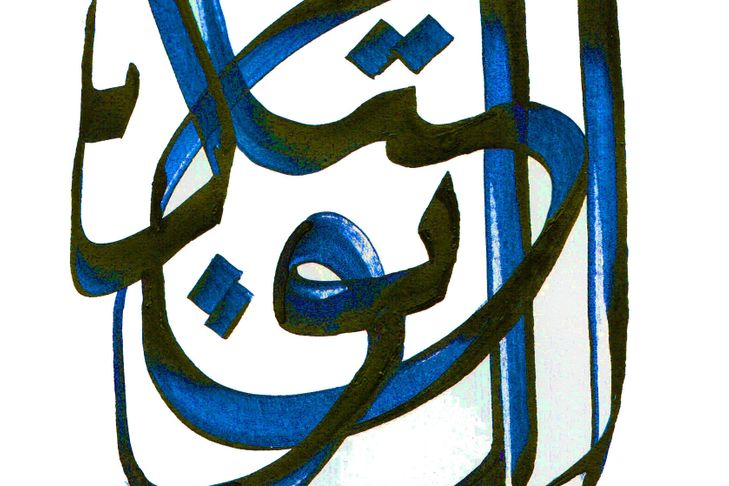
\includegraphics[width=\textwidth]{Images/image015.jpg}
« Le tawhid renvoie dans l'islam au dieu « un ». Mais la notion est
évolutive. Dans le Coran, le dieu local,~\emph{« protecteur du point
d'eau de La Mekke »}, se mue rapidement en dieu créateur, qui se suffit
à lui-même et n'a pas d'associé. C'est une manière de déligitimer les
trois déesses locales qui étaient supposées protéger les déplacements.
Plus tard, sur la coupole du Rocher à Jérusalem, construite en 692, est
inscrit un verset coranique (Sourate 4, Verset 171) qui récuse la
Trinité, faisant simplement de Jésus, « Fils de Marie », le « messager »
qui précède Mohammed. On semble être dans un défi à l'empire byzantin.
Enfin, beaucoup plus tard, au milieu du XVIII\textsuperscript{e}~siècle,
le tawhid devient un enjeu interne à l'islam avec le mouvement sectaire
du wahhabisme qui combat avec virulence les courants mystiques de
l'islam qui sont accusés « d'associer » d'autres divinités à Dieu. » \sn{Jacqueline Chabbi}



« Pour dessiner l'unité, j'ai utilisé dans cette calligraphie la forme
du carré. Lors de mes premiers essais, je faisais plutôt des cercles.
Là, j'ai déformé une des lettres (le h) pour la relier avec les autres
et les faire entrer toutes dans un carré. J'ai agrandi cette lettre
jusqu'à ce qu'elle enlace les autres lettres, comme dans un souffle. En
calligraphie, le souffle est important. Tous les calligraphes
travaillent sur le souffle. Quand on fait le geste, on coupe son
souffle. Quand on va à l'encrier, on reprend souffle. » \sn{Hassan Massoudy}



Le musulman, quand il récite la \emph{šahāda} ou quand il prêche, lève
l'index signifiant sa foi en Dieu un. À sa mort il est mis dans un
linceul, les mains jointes, et parfois, l'index droit désuni des autres
doigts de la main (parfois il est tourné vers le ciel).



\vide{adorer-dieu}{%
\subsubsection{{Adorer Dieu
}}\label{adorer-dieu}}

Affirmant que Dieu est unique, le musulman récite quotidiennement la
sourate 112 intitulée, \emph{al-iḫlaṣ} que l'on traduit souvent par «~le
culte pur~».


\begin{table}[h!]
\resizebox{\textwidth}{!}{%

\begin{tabular}{p{7cm}p{7cm}}
1. Dis: «Il est Allah, Unique.
&

\TArabe{بِسْمِ اللَّهِ الرَّحْمَنِ الرَّحِيمِ}

\TArabe{قُلْ هُوَ اللَّهُ أَحَدٌ}
\\
2. Allah, Le Seul à être imploré pour ce que nous désirons.
&
\TArabe{اللَّهُ الصَّمَدُ}
\\

3. Il n'a jamais engendré, n'a pas été engendré non plus.
& 
\TArabe{لَمْ يَلِدْ وَلَمْ يُولَدْ}
\\
4. Et nul n'est égal à Lui».
&
\TArabe{وَلَمْ يَكُنْ لَهُ كُفُوًا أَحَدٌ} \\

\end{tabular}%
}
\caption{sourate 112 , \emph{al-iḫlaṣ}, «~le
culte pur~»}
\end{table}



Au cours de l'histoire, cette sourate 112 a été invoquée par des
penseurs musulmans dans le cadre de \textbf{polémiques contre les
chrétiens}. Mais il faut noter qu'elle n'était pas, à son origine,
destinée à réfuter la croyance chrétienne. Elle est un \emph{credo}
contre le polythéisme.

L'affirmation d'un Dieu unique implique pour les musulmans que Dieu
existe. Il manifeste son existence dans des signes (\emph{āyāt},\TArabe{ آيات)},
ceux de la création, ceux du Livre qu'il a révélé.

Dire que Dieu est `un' implique que l'adoration revient à Lui seul. Seul
devant Lui le croyant se prosterne. La\emph{ʿibāda}, l'adoration, la
soumission totale, lui revient.

Si l'on refait un peu d'arabe vous voyez que la racine de \emph{ʿibāda}
est ʿa.Ba.Da. Vous la retrouvez dans le mot ʿAbd-Allāh\ldots{} qui
signifie serviteur, soumis, adorateur de Dieu.


\begin{Def}[Taghut]
{Taghut~(ar. \TArabe{طاغوت} ), ṭāġūt. Plusieurs~: Ṭawāġīt. Au sens large~: "aller au-delà de la mesure" ou désignant une "hauteur" ou un "sommet" de ṭāġiyah \TArabe{ طاغية} lit. tyran) est~une terminologie islamique~désignant un centre de culte autre que~Dieu.}
\end{Def}

La pensée musulmane est fondamentalement une pensée du Dieu unique~; la
prédication ne cessera d'attirer l'attention sur les idoles qui
s'immiscent dans l'islam au cours de l'histoire. Les grands réformateurs
de l'islam partent toujours de l'unicité divine. Ainsi, par exemple, au
XII\textsuperscript{e} siècle, la dynastie des Almohades instaurée au
Maroc s'appuie sur la doctrine d'Ibn Tumart (m.~1128). Ils se font
appeler les \emph{muwahhidūn}, c'est-à-dire les partisans de l'unicité,
les monothéistes, les unitariens.

\vide{notice-biographique-ibn-tumart-1080-1130}{%
\subsubsection{Notice biographique -- Ibn Tumart
(1080-1130)}\label{notice-biographique-ibn-tumart-1080-1130}}




C'est un personnage curieux qui après
avoir étudié en Andalousie et à Bagdad la doctrine d'al-Ašʿarī
(al-Ġazālī est aussi disciple d'al-Ašʿarī), revient dans son pays natal,
le haut Atlas et prêche un monothéisme rigoureux et réformateur. Dans
les montagnes, il va constituer un État disposant d'une armée, unie par
une doctrine religieuse rigoriste. Pour lui, toute forme de
divertissement est idolâtrie et contrevient à l'islam pur. Le \emph{dār
al-islām} (terre d'islam) ne saurait en ces conditions accueillir sur
son territoire des communautés religieuses non musulmanes. C'est de son
époque que l'on date la fin des communautés chrétiennes au Maghreb.
Ainsi, il condamne l'écoute de la musique qui éloigne de l'adoration qui
est due à Dieu. Son rigorisme moral lui attira bien des ennemis. À la
fin de sa vie, il se proclame Imam, Mahdi. Comme nous le verrons dans la
prochaine leçon, c'est une doctrine essentiellement šīʿite.



\textit{{Pour plus de détails, vous pouvez lire sa
biographie issue de \emph{l'Encyclopédie berbère}, p.3604-3606.
}}
 

De même, au 18\textsuperscript{ème} siècle, dans la péninsule arabique,
ʿAbd al-Wahhab entreprend une réforme de l'islam. Il s'agit avant tout
de s'attaquer à la prolifération de la superstition et de
l'associationnisme (\emph{širk}) dans la péninsule. Dans son Livre
\emph{Kitāb al-tawḥīd}, il invoque la nécessité d'adorer Dieu seul et de
rejeter le \emph{ṭāġūt} (\textbf{\TArabe{طاغوت}})\textbf{,} c'est-à-dire
tout ce qui est adoré en dehors de Dieu et qui contredit la Loi
islamique. Il y mentionne par exemple le port d'un bracelet pour
conjurer le mal, le port de talisman, etc.

Aujourd'hui, la propagande de Daesh a témoigné qu'il s'agit aussi d'un
mouvement unitarien rigoriste. L'État islamique est dans la même ligne
que celle d'un Ibn Tumart. La destruction des mausolées, des statues
antiques, des mosquées abritant le tombeau de saints sont les
conséquences de l'affirmation du \emph{tawḥīd} tel que défini par ʿAbd
al-Wahhab dans son \emph{Livre de l'unicité divine}~: pour lui, il ne
suffit pas d'affirmer que Dieu est unique (\emph{tawḥīd al-rubūbiyya})~;
cette affirmation doit aussi se mettre en œuvre dans la pratique en
n'adorant que Dieu seul (\emph{tawḥīd al-ulūhiyya}) et en combattant
toute forme d'idolâtrie. La croyance en l'intercession des prophètes ou
des saints sont vues comme autant de formes d'associationnisme à
combattre. D'où la destruction des mausolées.

\begin{marginfigure}

\includegraphics[width=\textwidth]{Images/image072.jpg}
\caption{Partisans de l'État islamique, l'index levé Les drapeaux mentionnent la šahāda}
\end{marginfigure}



\paragraph{ʿAbd al-Wahhab et le
salafisme}

Mohammed ibn Abd al-Wahhab (1703-1792) est le «~père~» de la doctrine
salafiste moderne. \textbf{Le salafisme se caractérise par la volonté de
purger la pratique religieuse de ses particularités locales et des
«~innovations~» qui auraient altéré l'islam originel au fil des
siècles}\textbf{. Il refuse toute forme d'inculturation}. Ce retour à la
religion des origines, quel que soit le pays où l'islam est pratiqué,
est fondé sur une lecture littéraliste des versets du Coran et des
\emph{ḥadīṯs}. Les salafistes refusent toute légitimité aux professions
de foi des penseurs musulmans ou aux écoles de droit qui ont développé
une méthodologie propre.

Longtemps rejeté, considéré comme une secte, le salafisme semble avoir
gagné le terrain idéologique ces trente dernières années et a su
s'imposer dans les consciences comme étant le véritable islam.

Hamadi Redissi y a consacré un livre, \emph{Le pacte de Nadj} où il
montre l'alliance entre le politique et le religieux. Il écrit~: «~La
tradition sunnite s'est défendue avec une impitoyable virulence contre
le wahhabisme, dans une campagne impitoyable qui n'est pas sans rappeler
l'acharnement médiéval contre l'hétérodoxie {[}\ldots{]}. (Mais) tout se
passe comme si le wahhabisme avait réveillé dans la conscience assoupie
de l'islam un potentiel insoupçonné de vérité, qui n'attendait que son
heure pour se révéler au grand jour. Une triple alliance entre princes,
ulémas et marabouts lui a pourtant tenu vaillamment tête, du milieu du
XVIIIème siècle à la fin du XIXème~».

Attention, cependant, le salafisme a différentes formes selon les
époques. On distingue le salafisme piétiste du salafisme djihadiste ou
encore du salafisme politique.

\vide{le-danger-de-lassociationisme-ux161irk}{%
\subsubsection{Le danger de l'associationisme
(\emph{širk})}{}\label{le-danger-de-lassociationisme-ux161irk}}

\begin{Def}[širk]
Le grand danger qui guette le croyant est donc d'associer quelque chose
à Dieu. L'associationnisme se nomme en arabe le \emph{širk}.
\end{Def}

L'accusation de \emph{širk} a une portée religieuse et politique
puisqu'elle vise à exclure l'autre de la communauté et appelle à le
combattre. Le \emph{mušrik} est l'associationniste. Cette accusation est
celle dressée contre les non-musulmans (juifs, chrétiens, polythéistes)
mais aussi contre ceux qui au sein de l'islam sont considérés comme
infidèles au \emph{tawḥīd.}


\mn{Muhammad Ibn
Tumart~:~\TArabe{المهدي
محمد بن تومرت}), 
réformateur~musulman.
à la morale~rigoriste. Voir  p. \pageref{IbnToumart}}
Pour Ibn Tumart, celui qui écoute de la musique est donc un
\emph{mušrik}. Cela peut éclairer certains débats contemporains.

\paragraph{le širk comme arme politique}

Un des premiers exemples politiques dans l'histoire de l'islam de
l'instrumentalisation politique du širk appliquée à l'encontre d'autres
musulmans est celui des ḫāriğites envers `Alī à la suite de son
acceptation de l'arbitrage proposé par Mu`āwiya lors de la bataille de
Ṣiffīn en 657\sn{\textsc{~Al-ṬabarĪ,} \emph{Tārīḫ}, I, 3363.}.
L'accusation de širk est aussi le nœud de bien des controverses
doctrinales~: dans le débat sur le Coran incréé, les muʿtazilites ont
accusé de širk les ḥanbalites et tous ceux qui refusaient de croire que
le Coran est créé. Ils comparèrent leur position à celle des chrétiens
qui soutiennent que Jésus est le Verbe incréé de Dieu et ils affirmèrent 
«~qu'il n'y a pas de \textit{tawḥīd} chez ceux qui n'acceptent pas que le Coran
est créé~»~: «~leurs doctrines sont du pur \textit{kufr} et un \textit{širk} évident aux
yeux du Commandeur de la foi~»\sn{~\textsc{Al-ṬabarĪ,}
  \emph{Tārīḫ}, III, 1112-1132. Voir Joseph \textsc{Van Ess},
  \emph{Theologie und Geselschaft}, III, p.~452-456.}. 
  
  Ce débat
théologique sur le Coran a trouvé son prolongement dans la question des
attributs divins comme la Vérité, le Bien pur, la Sagesse. Pour les
muʿtazilites, les attributs doivent être rattachés à l'essence divine,
sinon cela revient à introduire de la pluralité en Dieu et contrevient
par conséquent à l'unicité divine. De même, les philosophes voient dans
les chapitres du \textit{kalām} sur cette question l'introduction d'accidents en
Dieu.

\paragraph{Qu'en est-il de l'expression dans le Coran~?} Puisque le \emph{širk} est
si important, il n'est pas inutile de voir ce qu'en dit le Coran\ldots{}
et à qui il applique la catégorie. Évidemment, la Sunna ne donnerait pas
les mêmes conclusions\ldots{} mais cela est une autre question.

Notons que dans le Coran, les gens du Livre (\emph{ahl al-kitāb})
{[}chrétiens, juifs, sabéens{]} ne sont jamais appelés \emph{mušrikūn}
mais \emph{kuffār} (S.2, 105~; 3, 186~; 5, 82~; 22, 17)\sn{~Ainsi,
  par exemple, S. 2, 105~: 
 
      «~Ceux d'entre les gens du Livre qui sont
  \emph{incrédules} et les polythéistes ne voudraient pas qu'un bienfait
  de votre Seigneur descende sur vous. Dieu accorde en particulier sa
  miséricorde à qui il veut. Dieu est le maître de la grâce
  incommensurable~».
 
 \TArabe{مَا يَوَدُّ الَّذِينَ كَفَرُوا \textbf{مِنْ أَهْلِ الْكِتَابِ}
  \textbf{وَلَا الْمُشْرِ}كِينَ أَنْ يُنَزَّلَ عَلَيْكُمْ مِنْ خَيْرٍ
  مِنْ رَبِّكُمْ وَاللَّهُ يَخْتَصُّ بِرَحْمَتِهِ مَنْ يَشَاءُ وَاللَّهُ
  ذُو الْف
 َضْلِ الْعَظِيمِ}
 }.

Pour le Coran, le \emph{mušrik} est celui
qui affirme que Dieu a pris des enfants (S. 19, 88), qui cherche refuge
dans les \emph{ǧinns} (S. 72, 6), qui soutient que les anges sont des
êtres divins (S. 53, 27-28). Le terme collectif \emph{mušrikūn} désigne
ceux qui refusent de reconnaître la prédication du prophète~; ils sont
ses adversaires sur le plan religieux, politique et moral en tant qu'ils
commettent des péchés. Le Coran démasque les racines `psychologiques' du
\emph{širk} dans le \emph{ẓann}, opinion emplie d'incertitude et de
doute, contraire à la science (\emph{ʿilm}).
\begin{quote}
    {S. 10, 66 : «~Ce
  qui est dans les cieux et sur la terre n'appartient-il pas à Dieu~?
  Que suivent donc ceux qui invoquent des associés en dehors de Dieu~?
  Ils ne suivent que des conjectures et ils se contentent de
  suppositions~»

  \TArabe{أَلَا إِنَّ لِلَّهِ مَنْ فِي السَّمَاوَاتِ وَمَنْ فِي الْأَرْضِ
  وَمَا يَتَّبِعُ الَّذِينَ يَدْعُونَ مِنْ دُونِ اللَّهِ شُرَكَاءَ إِنْ
  يَتَّبِعُونَ إِلَّا \textbf{الظَّنَّ} وَإِنْ هُمْ إِلَّا يَخْرُصُونَ}
  },

\end{quote}
mais aussi dans les passions (\emph{ahwāʾ}). Par suite, le \emph{širk}
est une manifestation du \emph{kufr}~: il en est son degré paroxystique.
Le \emph{mušrik} est donc un égaré (S.~4, 117), il est le jouet de Satan
et son associationnisme annule toute rétribution positive de ses œuvres
aussi bonnes soient-elles (S.~39, 65)
\begin{quote}
    {~S. 6, 88 : «~Voilà la
  Direction de Dieu. Il dirige qui il veut parmi ses serviteurs. S'ils
  avaient été polythéistes, leurs actions ne leur auraient été d'aucun
  profit~».

  \TArabe{ذَلِكَ هُدَى اللَّهِ يَهْدِي بِهِ مَنْ يَشَاءُ مِنْ عِبَادِهِ
  وَلَوْ أَشْرَكُوا لَحَبِطَ عَنْهُمْ مَا كَانُوا يَعْمَلُونَ}
  }.
\end{quote}

Le
verset S. 9, 5 affirme que l'associationniste doit être combattu jusqu'à
ce que mort s'ensuive, à moins qu'il ne se convertisse à l'islam --
exigence qui n'est pas requise pour les gens du Livre. Il est aussi dit
qu'il n'est qu'impureté (S.~9, 28)
{S.9, 28~:

  \TArabe{إِنَّمَا الْمُشْرِكُونَ نَجَسٌ}}.

Aux yeux de l'orthodoxie sunnite et šīʿite, il est la plus grande
injustice causée à Dieu, le péché majeur, celui qui théoriquement ne
peut être pardonné (S. 4, 48)
\begin{quote}
    {S. 4, 48 : «~Dieu ne pardonne pas
  qu'on lui associe quoi que ce soit~; il pardonne à qui il veut des
  péchés moins graves que celui-ci. Celui qui associe quoi que ce soit à
  Dieu commet un crime immense~».

  \TArabe{إِنَّ اللَّهَ لَا يَغْفِرُ أَنْ يُشْرَكَ بِهِ وَيَغْفِرُ مَا دُونَ
  ذَلِكَ لِمَنْ يَشَاءُ وَمَنْ يُشْرِكْ بِاللَّهِ فَقَدِ افْتَرَى
  إِثْمًا عَظِيمًا}}.

\end{quote}

\paragraph{širk et Soufisme } Si les soufis furent souvent accusés de \emph{širk}, il n'en demeure pas
moins que leur enseignement est profondément pénétré du \emph{tawḥīd}.
Ainsi, par exemple, la mystique Rābiʿa (m.185/801) chante son amour
absolu pour Dieu qui ne laisse en son cœur aucune place pour
Muḥammad\sn{~Annemarie \textsc{Schimmel,} "\emph{The Sufis and
  the Shahāda}" dans Richard G. \textsc{Hovannisian} and Speros
  \textsc{Vryonis}, \emph{Islam's understanding of itself}, Eighth
  Giorgio Levi della Vida Biennial Conference, May 1-3, 1981, Malibu,
  Undena Publications, 1983, p.~103-125.}~; al-Ḥallāǧ (m.~309/922) \sn{le
mystique de Bagdad qui fut crucifié en 922 alors qu'il disait «~Je suis
Dieu~» (\emph{sic~!}). On en reparlera dans le cours consacré au
soufisme p. \pageref{iii--grandes-figures-soufies}}
incrimine la récitation continuelle de la \emph{šahāda}.
\begin{quote}
    {~«~{[}Al-Ḥallāǧ{]}
  condamne, nous dit Louis Massignon, l'illusion criminelle de certains
  qui s'imaginent, en récitant la \emph{šahāda}, témoigner réellement
  que Dieu est unique~; c'est oser `s'associer à Dieu'. Car s'imaginer
  que l'on `unifie' Dieu, c'est affirmer son propre moi~» : Louis
  \textsc{Massignon}, \emph{La Passion de Husayn Ibn Mansûr Hallâj},
  \emph{op.cit}., t.3, p.~247.}
\end{quote}

Al-Šiblī (m.~334/945), le disciple
d'al-Ǧunayd, de renchérir plus tard en confessant à propos de l'appel à
la prière : \sn{\textsc{Al-QuŠayrĪ,} \emph{Al-Risālat
  al-qušayriyya}, p.~17.}.
\begin{quote}
    Si Tu ne l'avais pas ordonné je n'aurais invoqué le nom de
nul autre que Toi
\end{quote}
 Ainsi, en se vouant à l'amour pur et absolu
de Dieu, ils s'attachent à déloger et démasquer toute trace de
\emph{širk} dans la dévotion et les pratiques mauvaises pour accéder à
Dieu. Ḥasan al-Baṣrī, un autre grand mystique, contemporain de
Rābiʿa~disait : \sn{\textsc{Ibn Saʿd},
  \emph{Al-Ṭabaqāt al-kubrā}, Beyrouth, Dār Ṣādir, t. 26, p.~17.}
\begin{quote}
    «~Alors qu'il avait achevé de parler et s'apprêtait à se
lever, Ḥasan dit~: `Ô mon Dieu, tu vois nos cœurs emplis de \emph{širk},
d'orgueil (\emph{kubr}), d'hypocrisie (\emph{nifāq}), du désir double
d'être vu et entendu, d'hésitation et de doute envers ta religion. Ô toi
qui retourne les cœurs, affermis nos cœurs en ta religion et assure que
notre religion soit l'islam véritable~».
\end{quote}
 Un
célèbre \emph{ḥadīṯ} est à cet égard convoqué puisqu'il rapporte que le
\emph{širk} est aussi imperceptible que le rampement d'une fourmi noire
sur une roche noire\sn{~\textsc{Ibn Ḥanbal}, \emph{Al-Musnad},
  Vol. IV, p.~403 :~«~Ô gens, méfiez-vous de cet associationnisme, car
  il est plus caché que le rampement des fourmis ».}.


  \paragraph{Les degrés de l'associationisme}
  
  Ces subtilités plus ou moins reconnues, admises et précisées par les
courants de pensée, les théologiens et les mystiques, définissent ainsi
des distinctions quant à sa nature et ses degrés. Ainsi convient-il de
distinguer le \emph{širk al-akbar} qui consiste à donner des associés à
Dieu, à sacrifier pour les \emph{djins} ou à adorer un prophète, du
\emph{širk al-aṣġar} qui ne touche pas le \emph{tawḥīd} à sa base mais
l'altère. Les soufis, dans une formule paradoxale, en viennent à
signifier que «~l'essence du \emph{širk} est de penser que l'on est sans
\emph{širk}~»\sn{~\textsc{Al-Hujwírí}, \emph{The Kashf al-maḥjúb :
  the oldest Persian Treatise on Ṣúfiism}, translated by Reynold A.
  Nicholson, Leyden, Brill, London, Luzac and Co, 1911, p.~282.}. 
  
  
  Ibn
Taymiyya, quant à lui, distingue entre l'associationnisme relatif à la
divinité (\emph{širk al-ulūhiyya}) et l'associationnisme relatif à la
seigneurie (\emph{širk al-rubūbiyya})\sn{~\textsc{Ibn Taymiyya},
  \emph{Maǧmūʿ al-fatāwā}, édition Ibn Qāsim, t. 1, Rabat, Maktabat
  al-Maʿārif, 1401/1981, p.~88-89, traduction française de Yahya Michot,
  «~Entre la divinité et la seigneurialité, le polymorphisme de
  l'associationnisme (\emph{shirk})~», \emph{Le Musulman}, n°16, sept.-
  déc. 1991, Paris, p.~8-13.}. Rappelez-vous, nous avons vu un peu plus
haut cette distinction, mais cette fois, c'était à propos du
\emph{tawḥīd}, l'unicité. Le premier consiste à donner à Dieu un
semblable en son adoration, en son amour, en son espérance, en sa peur,
en son repentir. Le croyant se tourne vers des «~pareils~» qu'il sait
inférieurs à Dieu, mais à qui il octroie cependant la place qui revient
à Dieu. Dans l'évocation et l'adoption de ces semblables, le croyant
affirme que s'il associe à Dieu, c'est pour mieux s'en rapprocher. Cet
associationnisme peut être pardonné à celui qui se repent et qui
abandonne ces pratiques. Quant à l'associationnisme relatif à la
seigneurie, il consiste à accréditer la cause d'un effet à un autre que
Dieu. Or Dieu, comme l'enseignent ses plus beaux noms, est celui qui
gouverne, avilit ou rend puissant, redresse ou abaisse, donne ou
empêche~: il est cause de tout.

\vide{anges-et-duxe9mons}{%
\subsection{{Anges et démons\ldots{}
}\label{anges-et-duxe9mons}}

\vide{les-anges}{%
\subsubsection{Les anges}\label{les-anges}}

Les anges et les démons occupent une place importante dans le Coran et
le \emph{ḥadīṯ}. L'ange~se dit \emph{malak} et au pluriel,
\emph{malāʾika} (en hébreu~: \emph{melek}). On les décrit comme des
êtres intermédiaires entre Dieu et les hommes (S. 70, 4). Leur nature
est spirituelle. Dans le \emph{ḥadīṯ}, ils sont dits asexués et
impeccables (c'est-à-dire sans péchés).

On trouve dans le Coran le nom de certains anges~: Ǧibrîl / Gabriel (S.
2, 97-98), Mīkāl / Michel (S.2, 98) et Mālik, l'ange chargé de l'enfer
(S. 43, 77).

Le Coran décrit le rôle qu'ils jouent. Ce sont~:

\begin{itemize}
\item
  des adorateurs
\item
  des modèles d'obéissance
\item
  des messagers que Dieu envoie aux hommes pour leur apporter ses
  ordres. Ils annoncent des naissances miraculeuses~: Isaac à Ibrahim,
  Jean-Baptiste à Zacharie, Jésus à Marie (S. 19, 16-19).
\item
  Ils sont les gardiens de l'Écriture mère. Gabriel est aussi appelé
  \emph{rūh}, c'est-à-dire esprit.
\item
  ils conservent et enregistrent les actions, bonnes ou mauvaises des
  hommes (\emph{ḥafiẓa}~: apprendre par cœur). En revanche, on ne peut
  pas parler d'ange gardien.
\item
  Ils interviennent dans les combats contre les infidèles.
\item
  Munkar et Nakīr sont les deux anges de l'interrogatoire du tombeau.
\end{itemize}

\vide{les-duxe9mons}{%
\subsubsection{Les démons}\label{les-duxe9mons}}

On parle des démons (\emph{šayāṭīn}) et du démon (\emph{al-šayṭān})
identifié à Iblīs à qui Dieu a demandé de se prosterner devant l'homme
créé d'argile et qui a refusé, parce que lui, il était une créature de
feu~:

\begin{quote}
S.2, 34~: «~Et lorsque Nous demandâmes aux Anges de se prosterner devant
Adam, ils se prosternèrent à l'exception d'Iblis qui refusa, s'enfla
d'orgueil et fut parmi les infidèles~».


\TArabe{وَإِذْ قُلْنَا لِلْمَلَائِكَةِ اسْجُدُوا لِآَدَمَ فَسَجَدُوا إِلَّا
إِبْلِيسَ أَبَى وَاسْتَكْبَرَ وَكَانَ مِنَ الْكَافِرِينَ}
\end{quote}
Est-il un ange déchu~? La tradition hésite~: l'ange est impeccable~!
Alors, on en fait parfois un \emph{djinn} introduit subrepticement parmi
les anges. On dira aussi~: un ange par son espèce, mais djinn par son
comportement. Mais l'enjeu théologique n'est-il pas ailleurs~? Pourquoi
Dieu a-t-il demandé aux anges de se prosterner devant Adam~?

\begin{itemize}
\item
  Dieu dans les versets précédents informe avoir enseigné à Adam tous
  les noms~; Il a donc un mérite spécial, particulier. Et les anges ne
  le voient pas. Pour que les anges comprennent ce mérite, Dieu demande
  que les anges se prosternent devant l'homme.
\item
  Il y a un enseignement spirituel pour les hommes eux-mêmes~: Quand tu
  ne sais pas pourquoi, sache que c'est parce que ta raison est
  limitée~: tout est limité en toi~: ta vue est limitée~: tu ne vois pas
  les anges, tu ne vois pas le mouvement du vent. Ton ouïe est limitée~:
  tu n'entends pas les djinns parler entre eux. De même pour la raison.
  Donc l'homme doit accepter les choses telles que Dieu les présente),
  telles qu'il les fait. Il doit accepter aussi l'ordre religieux.
\item
  Mais on a d'autres interprétations. Ainsi, pour le mystique al-Hallāǧ
  (m.922) cité déjà ci-dessus, Iblīs refuse de se prosterner devant
  l'homme car la prosternation n'est vouée qu'à Dieu seul. C'est par
  fidélité au \emph{tawḥīd} qu'il refuse. Mais justement, poursuit
  al-Hallāǧ, si Dieu demande cette prosternation, n'est-ce pas parce
  qu'il a divinisé l'homme en insufflant son esprit en lui~et en
  l'établissant \emph{ḫalīf} (calife) ? Al-Hallāǧ fut condamné à mort et
  crucifié pour ses théories incarnationnistes. On voit ici comment
  elles se fondent sur une interprétation du Coran qui n'est pas sans
  rigueur et cohérence.
\end{itemize}

\vide{les-livres}{%
\subsection{1.3 Les Livres}\label{les-livres}}

\vide{quels-livres-ruxe9vuxe9luxe9s}{%
\subsubsection{Quels livres révélés~?
}}\label{quels-livres-ruxe9vuxe9luxe9s}}

On trouve dans le Coran les mentions «~les livres~» (\emph{kutub}) ou
les feuillets (\emph{ṣuḥuf}) qui concernent les différentes révélations
du Livre envoyées aux prophètes. Elles sont nombreuses~comme l'indique
le verset S. 4, 163~:

\begin{quote}
«~Nous t'avons fait une révélation comme Nous fîmes à Noé et aux
prophètes après lui. Et Nous avons fait révélation à Abraham, à Ismaël,
à Isaac, à Jacob, aux tribus, à Jésus, à Job, à Aaron et à Salomon, et
Nous avons donné le Zabūr (les psaumes) à David~».

\TArabe{إِنَّا أَوْحَيْنَا إِلَيْكَ كَمَا أَوْحَيْنَا إِلَى نُوحٍ
وَالنَّبِيِّينَ مِنْ بَعْدِهِ وَأَوْحَيْنَا إِلَى إِبْرَاهِيمَ
وَإِسْمَاعِيلَ وَإِسْحَاقَ وَيَعْقُوبَ وَالْأَسْبَاطِ وَعِيسَى
وَأَيُّوبَ وَيُونُسَ وَهَارُونَ وَسُلَيْمَانَ وَآَتَيْنَا دَاوُودَ
زَبُورًا}
\end{quote}

De plus, on trouve les mentions précises de quatre écritures, à côté
bien sûr de celle du Coran~:

\begin{itemize}
\item
  La Thora, le mot apparait 16 fois dans le Coran, elle est le livre
  révélé à Moïse.
\item
  L'Évangile, (\emph{al-Inǧīl}) cité à douze reprises dans le Coran, et
  qui a été transmis à Jésus.
\item
  Les Psaumes (\emph{al-zabūr}) (S.4, 163~; 17, 55~; 21, 105)
\item
  Les feuillets (\emph{suhūf}) d'Abraham
\end{itemize}

\vide{la-question-de-la-falsification-taux1e25rux12bf}{%
\subsubsection{{La question de la falsification
(\emph{taḥrīf})
}}\label{la-question-de-la-falsification-taux1e25rux12bf}}

Nous avons déjà rencontré la théorie de la falsification des Écritures
et ses manifestations. Il convient ici de préciser qu'elle est
progressive et qu'elle donne lieu à des positions juridiques
différentes. Pour le coup, nous aborderons ce point dans le chapitre sur
le \emph{fiqh}, le droit musulman. Nous nous demanderons si l'on peut
s'appuyer sur ces Écritures pour en tirer des conséquences ou des
justifications légales. Certains savants ont fait remarquer que la
falsification portait non pas sur le texte du verset mais sur
l'interprétation qu'en proposaient les juifs et les chrétiens.

Pour l'heure, remarquons que la pluralité des Évangiles a été perçue
comme incompatible avec l'idée de révélation (\emph{tanzīl}) telle
qu'elle est comprise en islam. Dieu ne révèle pas des livres à un
prophète, mais un livre.

Dans le cadre de cette théorie de la falsification et de la
confrontation avec les juifs ou les chrétiens, certains théologiens
musulmans ont écrit des réfutations des écritures bibliques. Une des
plus connues est à cet égard celle d'Ibn Ḥazm (m. 1064). \label{Theol:IbnHazm2}

\paragraph{Notice biographique -- Ibn Ḥazm (m.1064)}

Ce théologien andalou, fondateur de l'école ẓahirite, c'est-à-dire
littéraliste, a été cité par Benoît XVI dans sa
\href{http://w2.vatican.va/content/benedict-xvi/fr/speeches/2006/september/documents/hf\_ben-xvi\_spe_20060912\_university-regensburg.html}{conférence
dite de Ratisbonne} en 2006. Dans son introduction, le pape parle du
Dieu d'Ibn Hazm qui n'est tenu ni à nous dire la vérité ni à faire le
bien. Une note renvoie aux travaux de Roger Arnaldez sur cet auteur.


\paragraph{Evangile de Barnabé}
Sur la base de la théorie de la falsification, on trouve en islam l'idée
qu'il existe un véritable évangile, transmis à Jésus, dans lequel Jésus
annonce explicitement la venue de Muḥammad. Cet Évangile n'est pas celui
de Matthieu, ni celui de Marc, ni de Luc et ni de Jean et il a été
détruit par les chrétiens. Cependant, un manuscrit a été retrouvé au
XVI\textsuperscript{e} siècle portant le titre «~Véritable Évangile de
Jésus~». Il s'agit de \textbf{l'Évangile de Barnabé}. Aujourd'hui, la
référence à cet Évangile a lieu essentiellement dans le cadre de
l'apologétique islamique. Pour autant, il n'est pas une source de droit
islamique. Il faut aussi noter que le Père Jacques Jomier a montré qu'il
s'agissait de l'œuvre d'un faussaire, probablement un moine converti à
l'islam\sn{~Jacques \textsc{Jomier}, «~L'Évangile selon Barnabé~»,
  dans \emph{MIDEO}, VI, Le Caire, 1959-1961, p. 137-226. Via le
  catalogue de la bibliothèque de l'IDEO du Caire vous avez accès à tous
  les articles du MIDEO. Pour celui qui nous concerne, c'est ici~:
  \url{https://alkindi.ideo-cairo.org/append_pdf/iu451.pdf/66561}}.

\vide{le-prophuxe9tisme-ou-le-monoprophuxe9tisme-musulman}{%
\subsection{Le prophétisme ou le monoprophétisme
musulman}\label{le-prophuxe9tisme-ou-le-monoprophuxe9tisme-musulman}}

Dans le Coran, les prophètes se succèdent au cours de l'histoire et sont
envoyés par Dieu à différentes nations afin que le message divin
parvienne jusqu'aux confins de la terre. Le Coran utilise deux termes
pour les désigner.

\begin{Def}[nabī et rasūl]
 Il distingue~:

\begin{itemize}
\item
  le \emph{nabī}, du verbe \emph{anba'a}, qui est chargé d'enseigner à
  son peuple l'existence du Dieu unique, l'obligation de Lui obéir et de
  n'adorer que Lui,
\item
  le \emph{rasūl}, du verbe \emph{arsala}, l'apôtre de Dieu, mandaté par
  Dieu pour transmettre la Loi religieuse (\emph{šarî`a}) qui conduira
  les hommes dans la voie droite
\end{itemize}
\end{Def}
{~On trouve une résonance de
    cette distinction dans le Nouveau Testament entre \foreignlanguage{greek}{προφἠτης}~et \foreignlanguage{greek}{
    απóστολος}~:~~«~C'est pourquoi la Sagesse de Dieu a dit~:
    «~J'enverrai vers eux des prophètes et des apôtres~» (\emph{Lc} 11,
    49). La préséance des apôtres sur les prophètes se retrouve dans la
    littérature patristique~: pour Théodore de Cyrus, le prophète est
    envoyé à une nation tandis que l'apôtre est envoyé au monde entier,
    dans PG 81, col. 844. Pour Jean Chrysostome, l'apôtre est de plus
    grande importance que le prophète, dans PG 57, col. 231 et si le
    prophète n'est pas toujours apôtre, l'apôtre, lui est toujours
    prophète~dans PG 51, col. 92. On note aussi chez les Pères une
    tendance à appeler apôtres ceux qui ne sont traditionnellement
    considérés que comme prophètes~: C'est le cas d'Isaïe ou de
    Jean-Baptiste appelé par Origène apôtres, dans PG 14, col. 786~:
    voir Arent Jan \textsc{Wensinck}.}.

Comme dans la Bible, l'apôtre est prophète, mais le prophète n'est pas
forcément apôtre\sn{`Abd al-Qâhir \textsc{al-Baġd}Â\textsc{d}Î,
  \emph{Uṣûl al-dîn}, Istanbul, s.d., p. 154.}. Le \emph{rasūl} est le
premier à être pleinement soumis à cette loi. Le Coran multiplie le
nombre de prophètes qui se succèdent d'Adam à Muḥammad (S. 23, 44) et
qui ne défaillent jamais devant leur mission. La question de la
non-défaillance et de l'inerrance du prophète est un thème fondamental
en islam. On trouve l'idée de l'impeccabilité (\emph{`iṣma})\sn{Le
  Coran ne contient aucun témoignage de l'impeccabilité (\emph{ʿiṣma},
  عصمة) des Prophètes, y compris eu égard à Muḥammad et les traces d'une
  telle affirmation dans la \emph{Sunna} y sont rares. La seule formule
  explicite se trouve dans le \emph{Musnad} d'Ibn Ḥanbal~: «~Je ne
  serais pas digne que vous suiviez mon exemple, puisque je suis votre
  prophète, si je n'étais préservé (\emph{ma`ṣûm}) de Satan~».} du
Prophète que nous avons déjà traitée à propos de Muḥammad. Ici, il faut
la comprendre non au sens où il ne commettrait pas de péchés -- le Coran
rapporte le péché d'Adam\sn{~S. 20, 121~: «~Adam désobéit à son
  Seigneur, il était dans l'erreur~» et S. 7, 22~: «~{[}Satan{]} leur
  jura~: `\,`je suis, pour vous, un conseiller digne de confiance'\,' et
  il les fit tomber par séduction. Lorsqu'ils eurent goûté aux fruits de
  l'arbre, leur nudité leur apparut~».}, de Moïse\sn{S. 28, 16~à
  propos du meurtre commis par Moïse : «~{[}Moïse{]} dit~: `\,`Mon
  Seigneur~! Je me suis fait tort à moi-même, pardonne-moi~».}, de
David\sn{S. 38, 24~: «~David comprit que nous avions seulement
  voulu l'éprouver. Il demanda pardon à son Seigneur~; il tomba
  prosterné et se repentit~»}, et les fautes de Muḥammad\sn{S. 4,
  79~: «~Tout bien qui t'arrive vient de Dieu~; tout mal qui t'atteint
  vient de toi-même~».} -- mais dans le don qu'il a de transmettre le
message divin avec une fidélité parfaite (\emph{ṣidq}, \emph{tablīġ}).

«~Dieu {[}les{]} a choisis, de préférence aux mondes~» (S. 3, 33), le
verbe \emph{iṣṭafā} indique une élection divine. C'est aux prophètes que
Dieu fait connaître «~le secret de son mystère~» (S. 72, 26).

La figure d'Abraham occupe un statut à part car c'est elle qui façonne
le modèle type du prophète de l'islam. Il est l'ami (\emph{ḫalīl}) de
Dieu, un vrai croyant (\emph{ḥanīf}), un soumis (\emph{muslim}) (S.~4,
125). En ce sens, non seulement il est l'avertisseur, mais aussi le
modèle idéal du parfait serviteur de Dieu (\emph{ʿabd Allāh}) et donc le
guide de la Communauté des croyants.~

Les prophètes sont envoyés par Dieu pour être obéis (S. 4, 64), mais ils
sont tournés en dérision (S. 15, 11), traités de menteurs (S. 3, 184~;
S. 22, 42~; S. 23, 44, etc.) et leur message est accusé de n'être qu'un
amas de rêves (S. 21, 5). Rejetés pour être des poètes, des magiciens
(\emph{sāḥir}) ou des mages (\emph{maǧnūn}) (S. 21, 5), les prophètes
ont souffert la persécution, et certains furent tués (S. 2, 61~; 2, 87~;
2, 91~; etc.). Le Coran donne peu d'indications biographiques sur chaque
prophète dont il mentionne le nom. Cependant, à partir du
XI\textsuperscript{ème} siècle, des \emph{Histoires des Prophètes}
(\emph{Qisās al-anbiyā'}), largement inspirées des récits bibliques ou
apocryphes, contribuent à redonner vie à ces personnages et leur
confèrent une valeur profondément spirituelle.

Certains orientalistes (je pense notamment à Alfred-Louis de Prémarre et
Claude Gilliot) parlent de monoprophétisme pour désigner le phénomène de
la prophétie en islam dans la mesure où Dieu transmet toujours la même
révélation aux hommes, le même message.

\vide{eschatologie}{%
\subsection{{Eschatologie
}}\label{eschatologie}}

La question eschatologique est fondamentale. Rappelez-vous, Muḥammad a
commencé la transmission des sourates avec cet appel à la conversion car
la fin des temps était proche. Nous y consacrerons un chapitre.

Notons d'ores et déjà que les Traités d'eschatologie musulmane à
l'exemple du \emph{Livre de la mort et de l'au-delà} d'al-Ġazālī
distinguent plusieurs étapes~: celle du Jour de la Résurrection, celle
du Jour du Grand Rassemblement, celle du Jour du Jugement. On y décrit
l'enfer, le paradis, mais aussi un lieu étrange~: \emph{al-aʿrāf}, sorte
de lieu transitoire. Le dernier chapitre sera consacré à l'eschatologie
musulmane. Nous nous quitterons donc avec les fins dernières, histoire
de nous dire que ce dernier chapitre ne sera qu'un au revoir.

\vide{libertuxe9-et-pruxe9destination}{%
\subsection{Liberté et prédestination
}{}\label{libertuxe9-et-pruxe9destination}}

Enfin la question de la prédestination (\emph{al-qadar}) fait aussi,
pour certains courants, partie des croyances musulmanes. Pour autant,
elle n'est pas sans poser problèmes théologiques et divergences
d'écoles. Car qu'en est-il de la liberté de l'individu si tout est écrit
d'avance (\emph{maktūb})~? L'acte humain est-il libre~?

Qu'en est-il de la liberté de l'infidèle, du mécréant, si Dieu avait
voulu qu'il soit mécréant~?

Et dans ce cas, pourquoi Dieu veut-il la mécréance~(\emph{kufr}) s'il
sait que le mécréant ira en enfer~? Dieu veut donc qu'il y ait des
hommes qui aillent en enfer et d'autres au paradis~? Et pourquoi a-t-il
choisi celui-ci et non celui-là~? De grandes questions, n'est-ce pas~? À
ce stade, je me contente de les poser. Mais sachez qu'elles ont donné
lieu en islam à des débats passionnants et discutés. On en parle peu
aujourd'hui. La tradition a été mutilée dirait Ghaleb Bencheikh\ldots{}
et elle est devenue mutilante.


\mn{Vous pouvez consulter le débat donné sur «~Islam et
Démocratie~ entre Ghaleb Bencheikh et Alain Finkielkraut donnée le 21
avril
2014 dans le cadre du \emph{Global Forum For
Islamic
Reform}}



\vide{ii--les-principales-professions-de-foi}{%
\section{{Les principales professions de foi
}}\label{ii--les-principales-professions-de-foi}}

Si la \emph{šahāda} est l'attestation de foi, il est apparu nécessaire
de préciser la nature de cette foi. Dans ce cadre ont été élaborées des
professions de foi (\emph{ʿaqīda}). Comme nous le disions en
introduction, les premiers Credo sont peu bavards et il s'agit de
formules souvent ramassées clairement orientées contre des opinions de
groupes considérés comme déviants.

L'auteur de la profession de foi la plus ancienne qui nous soit parvenue
est inconnu. Son texte est nommé \emph{fiqh al-akbar I}. Par la suite,
on voit apparaître la profession de foi d'Abū Hanifa, une profession de
foi identifiée comme \emph{Fiqh al-akbar II} avant que ne soit rédigée
la fameuse profession de foi d'al-Ašʿarī, le grand maître.

Encore une fois, il faut bien voir que ces professions de foi sont des
réponses à des positions théologiques existantes au sein de la
communauté musulmane.

\vide{le-fiqh-al-akbar-i}{%
\subsection{{Le fiqh al-akbar I
}}\label{le-fiqh-al-akbar-i}}

Ce texte est constitué de dix articles\sn{\textsc{Wensinck},
  \emph{Muslim Creeds}, p. 103-104, traduit en français par Gardet,
  Anawati, \emph{Introduction à la théologie musulmane}, Paris, Vrin,
  2006 (1948), p. 139-140.}~:

\begin{quote}
«~Art.1 -- Nous ne considérons personne {[}parmi ceux qui professent
l'islam{]} comme infidèle en raison de sa foi ni ne nions sa foi.

Art. 2 -- Nous commandons le bien et prohibons le mal

Art. 3 -- Ce qui vous atteint ne pouvait pas vous manquer, ce qui vous
manque n'aurait pu vous atteindre.

Art. 4 -- Nous ne désavouons aucun des Compagnons de l'Apôtre d'Allāh ni
n'adhérons à l'un d'eux exclusivement.

Art. 5 -- Nous laissons à Dieu la question de `Uthmān et de `Alī, Lui
seul connaît les choses secrètes et cachées.

Art. 6 -- La connaissance (\emph{fiqh}) dans les questions de religion
est meilleure que celle concernant la Loi.

Art. 7 -- La différence d'opinions dans la communauté est un bienfait de
Dieu

Art. 8 -- Quiconque croit ce qu'il doit croire mais qui dit~: je ne sais
pas si Moïse et Jésus sont bien des envoyés, est un infidèle.

Art. 9 -- Quiconque affirme qu'il ne sait pas si Allāh est au ciel ou en
enfer est un infidèle.

Art. 10 -- Quiconque dit qu'il ne connait pas le châtiment de la tombe
appartient à la secte des jahmites qui est vouée à la perdition~».
\end{quote}
Cette profession de foi peut être désarmante. Il n'est pas fait mention
des anges, ni du \emph{tawḥīd}, ni des Écritures. En revanche, il est
bien question des prophètes et de l'eschatologie. Les articles semblent
explicitement s'opposer et dénoncer certaines idées ou factions.
L'article 1 vise par exemple les ḫariǧites pour qui le pécheur ne peut
être considéré comme musulman. L'article 4 concerne les partisans de
ʿAlī qui dénient toute autorité aux premiers califes, etc.

\vide{le-fiqh-al-akbar-ii-la-profession-de-foi-dabux16b-hanifa}{%
\subsection{{Le fiqh al-akbar II~: la profession de
foi d'Abū Hanifa
}}\label{le-fiqh-al-akbar-ii-la-profession-de-foi-dabux16b-hanifa}}
\begin{Def}[Wasiyya - Profession de Foi]
Cette profession de foi est appelée \emph{Wasiyya}, Testament. Elle est
plus longue et plus aboutie.\mn{On trouvera une traduction en français de cette
profession de foi attribuée à Abū Hanifa (mais de qualité très
moyenne).
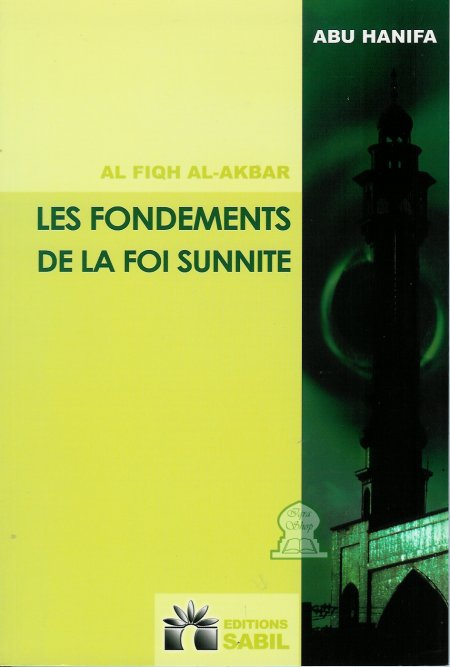
\includegraphics[width=3cm]{Images/image075.jpg}}
\end{Def}




{On en trouve sa traduction et son
commentaire en français.
}

Elle témoigne de l'émergence de nouvelles questions.

Par exemple, si vous prenez le premier article~: il y est dit que la foi
consiste à témoigner par la langue, l'assentiment du cœur et l'esprit~:
il ne suffit donc pas de dire, il faut croire à ce que l'on dit et aussi
comprendre ce que l'on dit. Certains diront que l'assentiment du cœur
suffit, et qu'il n'est pas nécessaire de prononcer la
\emph{šahāda}\ldots{} D'autres diront que le dire suffit aux yeux des
hommes, mais non aux yeux de Dieu\ldots{} Bref, ces professions de foi
sont les conséquences de questions théologiques.

De même, il est dit que la foi ne peut pas croître ou décroître. On a la
foi ou on ne l'a pas. Ce ne sera pas l'avis des \textbf{ašʿarites}.

Dans l'article 2, il est dit qu'un musulman qui commet un péché demeure
toujours musulman. Ici, l'article s'oppose explicitement aux
\emph{ḫariǧites} qui affirment le contraire et qui prônent un islam
d'une moralité très rigoureuse.

La \emph{Waṣiyya} se prononce aussi sur le caractère incréé du Coran
(art. 5) et donne des précisions sur l'eschatologie.

Les discussions se précisent toujours davantage et l'on voit aborder
toutes les grandes questions théologiques~: problème de la foi, du
\emph{tawḥīd}, du Coran, de la prédestination, de la prophétologie, de
l'eschatologie, du culte et du califat.






\subsection{Pour aller plus loin}

Daniel \textsc{Gimaret}, \emph{La doctrine d'al-Ash`arî}, Paris, Cerf,
Collection Patrimoine Islam, 1990.

C'est un excellent livre, mais il est très difficile, très technique.
Bref, pour les plus courageux, et surtout pour ceux que ces questions
passionnent.
 
 